\todo[inline]{figure out how to draw it}
	\begin{center}
		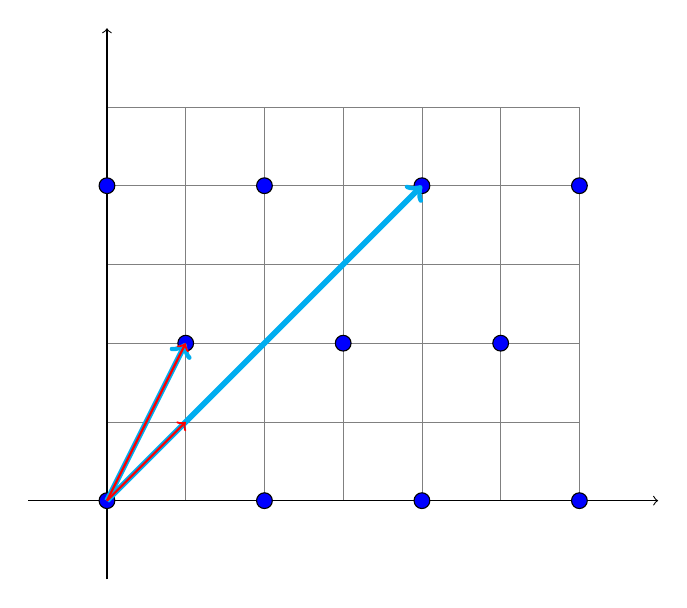
\begin{tikzpicture}
		\draw[help lines, line width=.2pt, step=1] (0,0) grid (6,5);
		\draw[->] (-1,0) -- (7,0);
		\draw[->] (0,-1) -- (0,6);
		\draw[fill=blue] (0,0) circle (0.1);
		\draw[fill=blue] (2,0) circle (0.1);
		\draw[fill=blue] (4,0) circle (0.1);
		\draw[fill=blue] (6,0) circle (0.1);
		\draw[fill=blue] (0,4) circle (0.1);
		\draw[fill=blue] (2,4) circle (0.1);
		\draw[fill=blue] (4,4) circle (0.1);
		\draw[fill=blue] (6,4) circle (0.1);
		\draw[fill=blue] (1,2) circle (0.1);
		\draw[fill=blue] (3,2) circle (0.1);
		\draw[fill=blue] (5,2) circle (0.1);
		\draw[->, cyan, line width=2pt] (0,0) -- (1,2);
		\draw[->, cyan, line width=2pt] (0,0) -- (4,4);
		\draw[->, red, thick] (0,0) -- (1,2);
		\draw[->, red, thick] (0,0) -- (1,1);
		\end{tikzpicture}
	\end{center}